\chapter{Numerical Experiments}   
\label{chap:numerical-experiments}

To be written.

\section{Section 1}
\label{sec:dyn-sec-1}

There are several way of adding pertubation to a problem 
- We can add noice to the paramterization of the problem 
- We can add noice to the curve itself 
- We can do some mapping of the paramterization, f.ex. \(I^2\)

Anyway, when looking into adding noice, it must be done either in the paramterization or in the curve itself. 

By adding noice to the paramterization we need to make sure that we still start and end in the same point, and that the paramterization still is monotone. When adding noice to the parameterization we still have the same curve, but the paramterization is different.

In contrast to adding noice to the paramterization, adding noice to the curve itself will change the curve. This means that we won't actually be able to reparameterize the curve to the original curve, as they will have different shape. 

Case 1: \(c = f(I + \epsilon) \)
Case 2: \(c = f(I) + \epsilon \)

For \(f(x) = x \) we have that the two cases are the same. 
While for \(f(x) = c \) we see that \(f(x + \epsilon) = c \neq c + \epsilon = f(x) + \epsilon \quad \forall \quad \epsilon \neq 0\)

Here we would want figures to show the difference between the two cases.

% Here we want a figure containing 2 subfigures, one for the continuous curve, where we place the parameterization on the curve, and one for the discrete curve.

\begin{figure}
    \centering
    \begin{subfigure}[b]{0.45\textwidth}
        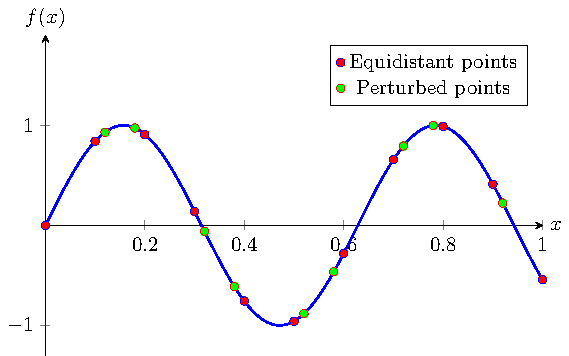
\includegraphics[width=\textwidth]{figures/perturbation-parameterization-cont/fig.pdf}
        \caption{}
        \label{fig:perturbation-parameterization-cont}
    \end{subfigure}
    \hfill
    \begin{subfigure}[b]{0.45\textwidth}
        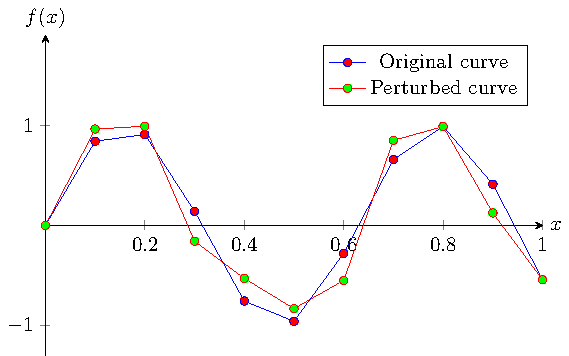
\includegraphics[width=\textwidth]{figures/perturbation-parameterization-disc/fig.pdf}
        \caption{}
        \label{fig:perturbation-parameterization-disc}
    \end{subfigure}
    \caption{Parameterization Perturbation for \( f(x) = \sin(10x) \): Continuous curve with uniform parameterization and its perturbed counterpart (a), versus the original and perturbed discrete curves at uniform steps (b), over \( x = [0, 1] \).}
    \label{fig:perturbation-parameterization}
\end{figure}


\begin{figure}
    \centering
    \begin{subfigure}[b]{0.45\textwidth}
        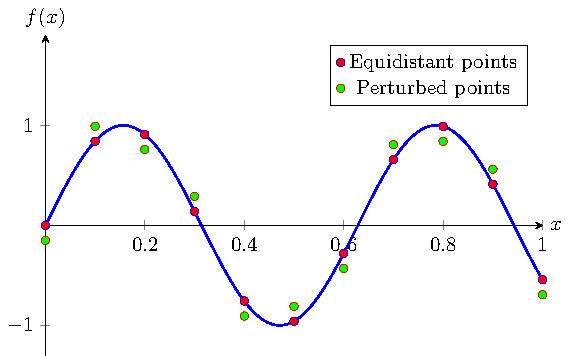
\includegraphics[width=\textwidth]{figures/perturbation-curve-cont/fig.pdf}
        \caption{}
        \label{fig:perturbation-curve-cont}
    \end{subfigure}
    \hfill
    \begin{subfigure}[b]{0.45\textwidth}
        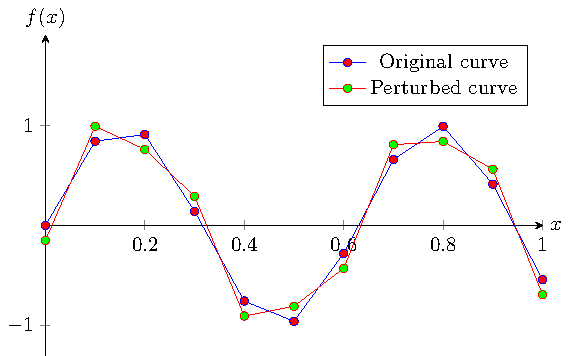
\includegraphics[width=\textwidth]{figures/perturbation-curve-disc/fig.pdf}
        \caption{}
        \label{fig:perturbation-curve-disc}
    \end{subfigure}
    \caption{Curve Perturbation for \( f(x) = \sin(10x) \): Impact of perturbations on the continuous curve (a), compared to the original and perturbed discrete curves at uniform steps (b), on \( x = [0, 1] \).}
    \label{fig:perturbation-curve}
\end{figure}

\begin{figure}
    \centering
    \begin{subfigure}[b]{0.45\textwidth}
        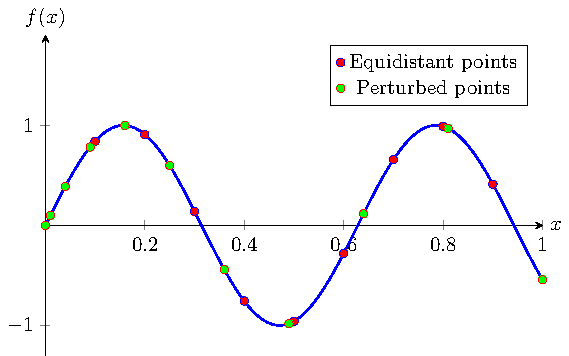
\includegraphics[width=\textwidth]{figures/perturbation-function-parameterization-cont/fig.pdf}
        \caption{}
        \label{fig:perturbation-square-parameterization-cont}
    \end{subfigure}
    \hfill
    \begin{subfigure}[b]{0.45\textwidth}
        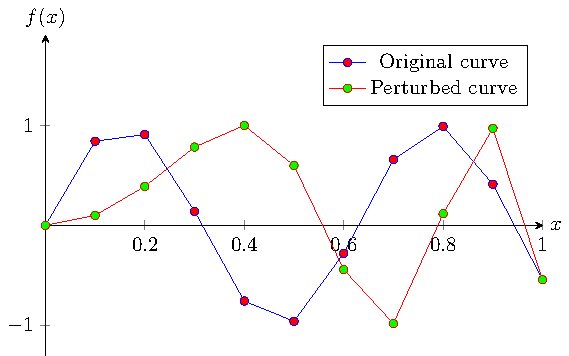
\includegraphics[width=\textwidth]{figures/perturbation-function-parameterization-disc/fig.pdf}
        \caption{}
        \label{fig:perturbation-square-parameterization-disc}
    \end{subfigure}
    \caption{Reparameterization Effect on \( f(x) = \sin(10x) \) with \( \hat{x} = x^2 \): Continuous curve under quadratic parameterization (a) and the corresponding perturbed discrete curve at uniform steps (b), on \( x = [0, 1] \).}
    \label{fig:perturbation-square-parameterization}
\end{figure}